% Chapter 4 from the standard thesis template
%   that contains an adv. example table and figure.
\chapter{NULLABOR: AN R PACKAGE FOR VISUAL STATISTICAL INFERENCE}\label{ch:nullabor}
\vspace{0.8cm}
\begin{center}
\large{A paper to be submitted to \it{Journal of Statistical Software}.}

\large{Niladri Roy Chowdhury, Hadley Wickham, Dianne Cook, Heike Hofmann, \\
Mahbubul Majumder}\\
\end{center}
\section{Introduction}\label{introduction}

The \textbf{nullabor} package provides a method of generating lineup
plots by randomly placing the true plot among a set of null plots for a
given null generating mechanism. This package also provides distance
metrics to calculate the distance between the plots in a lineup. The
diagnostic plots to compare one lineup to some other lineups can also
be drawn.

The null plots are generated from null datasets. The null datasets
correspond to a given null generating mechanism. The package provided
three different methods for generating null datasets.

\section{Generate null data with a specific
distribution}\label{generate-null-data-with-a-specific-distribution}

The \texttt{"null\_dist"} function takes as input a variable name of the
data and a particular distribution. This variable in the data is
substituted by random generations of the particular distribution. The
different distributions include beta, cauchy, chi-squared, exponential,
f, gamma, geometric, log-normal, lognormal, logistic, negative binomial,
normal, poisson, t and weibull. A list of parameters of distribution can
also be provided as input. In case it is not provided,
\texttt{"fitdistr"} is used to estimate the parameters from the given
data. The function \texttt{"null\_dist"} returns a function that given
the data generates a null data set.

\begin{Shaded}
\begin{Highlighting}[]
\KeywordTok{library}\NormalTok{(nullabor)}
\KeywordTok{head}\NormalTok{(}\KeywordTok{null_dist}\NormalTok{(}\StringTok{"mpg"}\NormalTok{, }\DataTypeTok{dist =} \StringTok{"normal"}\NormalTok{)(mtcars))}
\end{Highlighting}
\end{Shaded}

\begin{verbatim}
##                     mpg cyl disp  hp drat    wt  qsec vs am gear carb
## Mazda RX4         23.53   6  160 110 3.90 2.620 16.46  0  1    4    4
## Mazda RX4 Wag     19.98   6  160 110 3.90 2.875 17.02  0  1    4    4
## Datsun 710        30.34   4  108  93 3.85 2.320 18.61  1  1    4    1
## Hornet 4 Drive    21.30   6  258 110 3.08 3.215 19.44  1  0    3    1
## Hornet Sportabout 15.40   8  360 175 3.15 3.440 17.02  0  0    3    2
## Valiant           17.15   6  225 105 2.76 3.460 20.22  1  0    3    1
\end{verbatim}

\section{Generate null data by permuting a
variable}\label{generate-null-data-by-permuting-a-variable}

The \texttt{"null\_permute"} function takes as input a variable name of
the data. This variable is permuted to obtain the null dataset. The
function \texttt{"null\_dist"} returns a function that given the data
generates a null data set.

\begin{Shaded}
\begin{Highlighting}[]
\KeywordTok{head}\NormalTok{(}\KeywordTok{null_permute}\NormalTok{(}\StringTok{"mpg"}\NormalTok{)(mtcars))}
\end{Highlighting}
\end{Shaded}

\begin{verbatim}
##                    mpg cyl disp  hp drat    wt  qsec vs am gear carb
## Mazda RX4         15.5   6  160 110 3.90 2.620 16.46  0  1    4    4
## Mazda RX4 Wag     30.4   6  160 110 3.90 2.875 17.02  0  1    4    4
## Datsun 710        26.0   4  108  93 3.85 2.320 18.61  1  1    4    1
## Hornet 4 Drive    24.4   6  258 110 3.08 3.215 19.44  1  0    3    1
## Hornet Sportabout 27.3   8  360 175 3.15 3.440 17.02  0  0    3    2
## Valiant           10.4   6  225 105 2.76 3.460 20.22  1  0    3    1
\end{verbatim}

\section{Generate null data with null residuals from a
model}\label{generate-null-data-with-null-residuals-from-a-model}

The function \texttt{"null\_lm"} takes as input a model specification
formula as defined by \texttt{"lm"} and method for generating null
residuals from the model. The three built in methods are `rotate',
`pboot' and `boot' defined by \texttt{"resid\_rotate"},
\texttt{"resid\_pboot"} and \texttt{"resid\_boot"} respectively. The
function returns a function which given the data generates a null
dataset.

\begin{Shaded}
\begin{Highlighting}[]
\KeywordTok{head}\NormalTok{(}\KeywordTok{null_lm}\NormalTok{(wt~mpg, }\DataTypeTok{method =} \StringTok{'rotate'}\NormalTok{)(mtcars))}
\end{Highlighting}
\end{Shaded}

\begin{verbatim}
##                    mpg cyl disp  hp drat    wt  qsec vs am gear carb
## Mazda RX4         21.0   6  160 110 3.90 3.355 16.46  0  1    4    4
## Mazda RX4 Wag     21.0   6  160 110 3.90 2.940 17.02  0  1    4    4
## Datsun 710        22.8   4  108  93 3.85 3.849 18.61  1  1    4    1
## Hornet 4 Drive    21.4   6  258 110 3.08 3.770 19.44  1  0    3    1
## Hornet Sportabout 18.7   8  360 175 3.15 3.650 17.02  0  0    3    2
## Valiant           18.1   6  225 105 2.76 3.659 20.22  1  0    3    1
##                    .resid .fitted
## Mazda RX4          0.2659   3.089
## Mazda RX4 Wag     -0.1493   3.089
## Datsun 710         1.0137   2.836
## Hornet 4 Drive     0.7370   3.033
## Hornet Sportabout  0.2364   3.413
## Valiant            0.1610   3.498
\end{verbatim}

\section{The lineup protocol}\label{the-lineup-protocol}

In this protocol, the plot of the real data is randomly embedded amongst
a set of null plots. The matrix of plots is known as a lineup. The null
plots are generated by a method consistent with the null hypothesis. The
lineup is shown to an observer. If the observer can pick the real data
as different from the others, this puts weight on the statistical
significance of the structure in the plot. The \texttt{"lineup"}
function returns a set of generated null datasets and the real data
embedded randomly among these null datasets. The method of null
generation should be provided in the lineup function for the null
datasets to be generated automatically along with the real dataset. The
users also have the option of generating the null datasets themselves
and providing them in the \texttt{"lineup"} function. The position of
the real dataset can be left missing and the function picks the position
at random. The function then returns the position as an encrypted code.
The encrypted code is copied and pasted on the console to obtain the
true position of the plot.

\begin{Shaded}
\begin{Highlighting}[]
\KeywordTok{library}\NormalTok{(nullabor)}
\KeywordTok{head}\NormalTok{(}\KeywordTok{lineup}\NormalTok{(}\KeywordTok{null_permute}\NormalTok{(}\StringTok{"mpg"}\NormalTok{), mtcars), }\DecValTok{20}\NormalTok{)}
\end{Highlighting}
\end{Shaded}

\begin{verbatim}
## decrypt("jriG PHhH D5 QZXDhDZ5 Jl")
\end{verbatim}

\begin{verbatim}
##     mpg cyl  disp  hp drat    wt  qsec vs am gear carb .sample
## 1  14.7   6 160.0 110 3.90 2.620 16.46  0  1    4    4       1
## 2  22.8   6 160.0 110 3.90 2.875 17.02  0  1    4    4       1
## 3  21.4   4 108.0  93 3.85 2.320 18.61  1  1    4    1       1
## 4  33.9   6 258.0 110 3.08 3.215 19.44  1  0    3    1       1
## 5  16.4   8 360.0 175 3.15 3.440 17.02  0  0    3    2       1
## 6  10.4   6 225.0 105 2.76 3.460 20.22  1  0    3    1       1
## 7  15.0   8 360.0 245 3.21 3.570 15.84  0  0    3    4       1
## 8  19.7   4 146.7  62 3.69 3.190 20.00  1  0    4    2       1
## 9  32.4   4 140.8  95 3.92 3.150 22.90  1  0    4    2       1
## 10 18.7   6 167.6 123 3.92 3.440 18.30  1  0    4    4       1
## 11 14.3   6 167.6 123 3.92 3.440 18.90  1  0    4    4       1
## 12 10.4   8 275.8 180 3.07 4.070 17.40  0  0    3    3       1
## 13 17.8   8 275.8 180 3.07 3.730 17.60  0  0    3    3       1
## 14 22.8   8 275.8 180 3.07 3.780 18.00  0  0    3    3       1
## 15 26.0   8 472.0 205 2.93 5.250 17.98  0  0    3    4       1
## 16 27.3   8 460.0 215 3.00 5.424 17.82  0  0    3    4       1
## 17 19.2   8 440.0 230 3.23 5.345 17.42  0  0    3    4       1
## 18 30.4   4  78.7  66 4.08 2.200 19.47  1  1    4    1       1
## 19 13.3   4  75.7  52 4.93 1.615 18.52  1  1    4    2       1
## 20 15.8   4  71.1  65 4.22 1.835 19.90  1  1    4    1       1
\end{verbatim}

The lineup data can be then used to generate the lineup using
\textbf{ggplot2}. The lineup is shown to one or more observers who are
asked to identify the plot which is different. If the observer can
identify the plot of the real data correctly, we reject the null
hypothesis and conclude that the plot of the real data has stronger
structure than the null plots.

\begin{Shaded}
\begin{Highlighting}[]
\KeywordTok{qplot}\NormalTok{(mpg, wt, }\DataTypeTok{data =} \KeywordTok{lineup}\NormalTok{(}\KeywordTok{null_permute}\NormalTok{(}\StringTok{"mpg"}\NormalTok{), mtcars)) +}\StringTok{ }\KeywordTok{facet_wrap}\NormalTok{(~}\StringTok{ }\NormalTok{.sample)}
\end{Highlighting}
\end{Shaded}

\begin{verbatim}
## decrypt("jriG PHhH D5 QZXDhDZ5 4")
\end{verbatim}

\begin{figure*}[hbtp]
\begin{center}
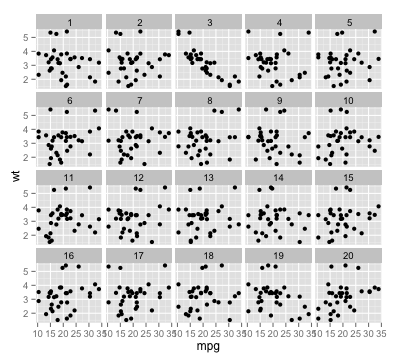
\includegraphics[scale=0.75]{unnamed-chunk-5.png}
\end{center}
\end{figure*}

\section{The Rorschach protocol}\label{the-rorschach-protocol}

The Rorschach protocol is used to calibrate the eyes for variation due
to sampling. The plots generated corresponds to the null datasets, data
that is consistent with a null hypothesis. The \texttt{"rorschach"}
function returns a set of null plots which are shown to observers to
calibrate their eyes with variation. Like the \texttt{"lineup"}
function, the null generating mechanism should be provided as an input
along with a real dataset. A probability can also be given as input
which dictates the chance of including the true data with null data.

\begin{Shaded}
\begin{Highlighting}[]
\KeywordTok{head}\NormalTok{(}\KeywordTok{rorschach}\NormalTok{(}\KeywordTok{null_permute}\NormalTok{(}\StringTok{"mpg"}\NormalTok{), mtcars, }\DataTypeTok{n =} \DecValTok{8}\NormalTok{, }\DataTypeTok{p =} \DecValTok{0}\NormalTok{), }\DecValTok{20}\NormalTok{)}
\end{Highlighting}
\end{Shaded}

\begin{verbatim}
##    .n  mpg cyl  disp  hp drat    wt  qsec vs am gear carb
## 1   1 21.0   6 160.0 110 3.90 2.620 16.46  0  1    4    4
## 2   1 15.5   6 160.0 110 3.90 2.875 17.02  0  1    4    4
## 3   1 10.4   4 108.0  93 3.85 2.320 18.61  1  1    4    1
## 4   1 19.2   6 258.0 110 3.08 3.215 19.44  1  0    3    1
## 5   1 13.3   8 360.0 175 3.15 3.440 17.02  0  0    3    2
## 6   1 15.0   6 225.0 105 2.76 3.460 20.22  1  0    3    1
## 7   1 18.7   8 360.0 245 3.21 3.570 15.84  0  0    3    4
## 8   1 10.4   4 146.7  62 3.69 3.190 20.00  1  0    4    2
## 9   1 14.7   4 140.8  95 3.92 3.150 22.90  1  0    4    2
## 10  1 15.2   6 167.6 123 3.92 3.440 18.30  1  0    4    4
## 11  1 26.0   6 167.6 123 3.92 3.440 18.90  1  0    4    4
## 12  1 21.5   8 275.8 180 3.07 4.070 17.40  0  0    3    3
## 13  1 21.0   8 275.8 180 3.07 3.730 17.60  0  0    3    3
## 14  1 17.8   8 275.8 180 3.07 3.780 18.00  0  0    3    3
## 15  1 17.3   8 472.0 205 2.93 5.250 17.98  0  0    3    4
## 16  1 14.3   8 460.0 215 3.00 5.424 17.82  0  0    3    4
## 17  1 18.1   8 440.0 230 3.23 5.345 17.42  0  0    3    4
## 18  1 22.8   4  78.7  66 4.08 2.200 19.47  1  1    4    1
## 19  1 16.4   4  75.7  52 4.93 1.615 18.52  1  1    4    2
## 20  1 19.2   4  71.1  65 4.22 1.835 19.90  1  1    4    1
\end{verbatim}

\section{Distance metrics}\label{distance-metrics}

There are five different distance metrics in \textbf{nullabor} package,
named \texttt{"bin\_dist"}, \texttt{"box\_dist"}, \texttt{"reg\_dist"},
\texttt{"sep\_dist"} and \texttt{"uni\_dist"}. The different distance
metrics are constructed so that they can identify the different
properties of the data. \texttt{"uni\_dist"} works for univariate data
while the others works for all types of bivariate data. Binned distance
is a generic distance which can be used in any situations while the
other distance metrics are constructed so that they can identify the
effect of graphical elements in a plot like an overlaid regression line
or presence of defined clusters. To calculate some of the metrics,
additional informations like a class variable or the number of bins
should be provided.

\subsection{Distance for univariate
data}\label{distance-for-univariate-data}

\texttt{"uni\_dist"} is a distance metric which calculates the euclidean
distance between the first four central moments of two univariate data.
A typical usage would be when one needs to calculate the distance
between the two histograms drawn from two datasets.

\begin{Shaded}
\begin{Highlighting}[]
\KeywordTok{library}\NormalTok{(nullabor)}
\KeywordTok{uni_dist}\NormalTok{(}\KeywordTok{rnorm}\NormalTok{(}\DecValTok{100}\NormalTok{), }\KeywordTok{rpois}\NormalTok{(}\DecValTok{100}\NormalTok{, }\DecValTok{2}\NormalTok{))}
\end{Highlighting}
\end{Shaded}

\begin{verbatim}
## [1] 2.309
\end{verbatim}

\subsection{Distance based on regression
parameters}\label{distance-based-on-regression-parameters}

\texttt{"reg\_dist"} is a distance metric which calculates the euclidean
distance between the regression parameters of a model fitted to one plot
and that of another plot. It is advisable to use this distance in
situations where a regression line is overlaid on a scatterplot.

\begin{Shaded}
\begin{Highlighting}[]
\KeywordTok{with}\NormalTok{(mtcars, }\KeywordTok{reg_dist}\NormalTok{(}\KeywordTok{data.frame}\NormalTok{(wt, mpg), }\KeywordTok{data.frame}\NormalTok{(}\KeywordTok{sample}\NormalTok{(wt), mpg)))}
\end{Highlighting}
\end{Shaded}

\begin{verbatim}
## [1] 618.1
\end{verbatim}

\subsection{Distance based on
boxplots}\label{distance-based-on-boxplots}

\texttt{"box\_dist"} is a distance metric which works for side-by-side
boxplots with two levels. The first quartile, median and the third
quartile are calculated for each box and the absolute distances of these
are calculated for the two boxes. \texttt{"box\_dist"} calculates the
euclidean distance between these absolute distances for the two plots.
The boxplot distance should be used in situations where a side-by-side
boxplot is used to compare the distribution of a variable at two
different levels.

\begin{Shaded}
\begin{Highlighting}[]
\KeywordTok{with}\NormalTok{(mtcars, }\KeywordTok{box_dist}\NormalTok{(}\KeywordTok{data.frame}\NormalTok{(}\KeywordTok{as.factor}\NormalTok{(am), mpg),  } \\
\KeywordTok{data.frame}\NormalTok{(}\KeywordTok{as.factor}\NormalTok{(}\KeywordTok{sample}\NormalTok{(am)), mpg)))}
\end{Highlighting}
\end{Shaded}

\begin{verbatim}
## [1] 11.81
\end{verbatim}

\subsection{Distance based on
separation}\label{distance-based-on-separation}

\texttt{"sep\_dist"} is a distance metric based on the separation
between clusters. The separation between clusters is defined by the
minimum distances of a point in the cluster to a point in another
cluster. The separation between the clusters for a given dataset is
calculated. An euclidean distance is calculated between the separation
for the given dataset and another dataset. The number of clusters in the
dataset should be provided. If not, the hierarchical clustering method
is used to obtain the clusters.

\begin{Shaded}
\begin{Highlighting}[]
\KeywordTok{with}\NormalTok{(mtcars, }\KeywordTok{sep_dist}\NormalTok{(}\KeywordTok{data.frame}\NormalTok{(wt, mpg,  }\KeywordTok{as.numeric}\NormalTok{(}\KeywordTok{as.factor}\NormalTok{(mtcars$cyl))), }\\
\KeywordTok{data.frame}\NormalTok{(}\KeywordTok{sample}\NormalTok{(wt), mpg,  }\KeywordTok{as.numeric}\NormalTok{(}\KeywordTok{as.factor}\NormalTok{(mtcars$cyl))), }\DataTypeTok{nclust =} \DecValTok{3}\NormalTok{))}
\end{Highlighting}
\end{Shaded}

\begin{verbatim}
## [1] 0.01651
\end{verbatim}

\subsection{Binned Distance}\label{binned-distance}

\texttt{"bin\_dist"} is a generic distance which works for any situation
for any dataset. For a given bivariate dataset, X and Y variables are
divided into p and q bins respectively to obtain pq cells. The number of
points falling in each cell are counted for a given dataset.
\texttt{"bin\_dist"} between two datasets calculates the euclidean
distance between the cell counts of these two data. The values of p and
q should be provided as arguments.

\begin{Shaded}
\begin{Highlighting}[]
\KeywordTok{with}\NormalTok{(mtcars, }\KeywordTok{bin_dist}\NormalTok{(}\KeywordTok{data.frame}\NormalTok{(wt, mpg), } \\
\KeywordTok{data.frame}\NormalTok{(}\KeywordTok{sample}\NormalTok{(wt), mpg), }\DataTypeTok{lineup.dat =} \OtherTok{NULL}\NormalTok{, }\DataTypeTok{X.bin =} \DecValTok{5}\NormalTok{, }\DataTypeTok{Y.bin =} \DecValTok{5}\NormalTok{))}
\end{Highlighting}
\end{Shaded}

\begin{verbatim}
## [1] 8.718
\end{verbatim}

\section{Calculating the mean distances for the plots in the
lineup}\label{calculating-the-mean-distances-for-the-plots-in-the-lineup}

It is interesting to see whether the true plot in a lineup is different
from all the null plots. To find this the distances between the true
plot and all the null plots are calculated and the mean of these
distances is calculated. Similarly, for each null plot, the distance
between the null plot and all the other null plots is calculated and
averaged to obtain the mean distance for each null plot.
\texttt{"calc\_mean\_dist"} calculates the mean distance corresponding
to each plot in the lineup. If the mean distance of the true plot is
larger than the mean distances of all the null plots, the lineup is
considered easy. If one of the null plots has a larger mean distance
than the true plot, the lineup is considered difficult.

\begin{Shaded}
\begin{Highlighting}[]
\KeywordTok{library}\NormalTok{(dplyr)}
\KeywordTok{calc_mean_dist}\NormalTok{(}\KeywordTok{lineup}\NormalTok{(}\KeywordTok{null_permute}\NormalTok{(}\StringTok{'mpg'}\NormalTok{), mtcars, }\DataTypeTok{pos =} \DecValTok{10}\NormalTok{), }\\
\DataTypeTok{var =} \KeywordTok{c}\NormalTok{(}\StringTok{'mpg'}\NormalTok{, }\StringTok{'wt'}\NormalTok{), }\DataTypeTok{met =} \StringTok{'reg_dist'}\NormalTok{, }\DataTypeTok{pos =} \DecValTok{10}\NormalTok{)}
\end{Highlighting}
\end{Shaded}

\begin{verbatim}
## Source: local data frame [20 x 2]
## 
##    plotno mean.dist
## 1       1    0.3030
## 2       2    0.3923
## 3       3    0.7187
## 4       4    0.3150
## 5       5    1.1514
## 6       6    0.2730
## 7       7    0.2857
## 8       8    0.8783
## 9       9    0.3466
## 10     10    9.1644
## 11     11    0.6400
## 12     12    0.4516
## 13     13    0.2748
## 14     14    0.3411
## 15     15    0.3779
## 16     16    0.2864
## 17     17    0.3057
## 18     18    0.2761
## 19     19    2.3577
## 20     20    0.3885
\end{verbatim}

\section{Calculating difference measure for
lineups}\label{calculating-difference-measure-for-lineups}

The mean distances for each plot in the lineup are obtained using
\texttt{"calc\_mean\_dist"}.\texttt{"calc\_diff"} calculates the
difference between the mean distance for the true plot and the maximum
mean distance for the null plots.

\begin{Shaded}
\begin{Highlighting}[]
\KeywordTok{calc_diff}\NormalTok{(}\KeywordTok{lineup}\NormalTok{(}\KeywordTok{null_permute}\NormalTok{(}\StringTok{'mpg'}\NormalTok{), mtcars, }\DataTypeTok{pos =} \DecValTok{10}\NormalTok{), }\DataTypeTok{var =} \KeywordTok{c}\NormalTok{(}\StringTok{'mpg'}\NormalTok{, }\StringTok{'wt'}\NormalTok{), } \\
\DataTypeTok{met =} \StringTok{'reg_dist'}\NormalTok{, }\DataTypeTok{dist.arg =} \OtherTok{NULL}\NormalTok{, }\DataTypeTok{pos =} \DecValTok{10}\NormalTok{)}
\end{Highlighting}
\end{Shaded}

\begin{verbatim}
## [1] 6.637
\end{verbatim}

\section{Optimum number of bins}\label{optimum-number-of-bins}

Binned distance is highly affected by the choice of the number of bins.
The number of bins is provided by the user and this can be subjective.
This motivates to design a way to select the optimum number of bins to
be used. \texttt{"opt\_diff"} finds the optimal number of bins in both x
and y direction which should be used to calculate the binned distance.
The binned distance is calculated for each combination of provided
choices of number of bins in x and y direction and finds the difference
using \texttt{"calc\_diff"} for each combination. The combination for
which the difference is maximum should be used.

\begin{Shaded}
\begin{Highlighting}[]
\KeywordTok{library}\NormalTok{(ggplot2)}
\NormalTok{opt.diff <-}\StringTok{ }\KeywordTok{opt_bin_diff}\NormalTok{(}\KeywordTok{lineup}\NormalTok{(}\KeywordTok{null_permute}\NormalTok{(}\StringTok{'mpg'}\NormalTok{), mtcars, }\DataTypeTok{pos =} \DecValTok{10}\NormalTok{), }\DataTypeTok{var =} \KeywordTok{c}\NormalTok{(}\StringTok{'mpg'}\NormalTok{, }\StringTok{'wt'}\NormalTok{), }\DecValTok{2}\NormalTok{, }\DecValTok{10}\NormalTok{, }\DecValTok{2}\NormalTok{, }\DecValTok{10}\NormalTok{, }\DataTypeTok{pos =} \DecValTok{10}\NormalTok{, }\DataTypeTok{plot =} \OtherTok{TRUE}\NormalTok{)}
\KeywordTok{head}\NormalTok{(opt.diff$dat)}
\end{Highlighting}
\end{Shaded}

\begin{verbatim}
## Source: local data frame [6 x 3]
## Groups: xbins
## 
##   xbins ybins    Diff
## 1     2     2 -1.1123
## 2     2     3 -1.1023
## 3     2     4 -0.7199
## 4     2     5 -0.7199
## 5     2     6 -1.3007
## 6     2     7 -0.7199
\end{verbatim}

\begin{Shaded}
\begin{Highlighting}[]
\NormalTok{opt.diff$p}
\end{Highlighting}
\end{Shaded}

\begin{figure*}[hbtp]
\begin{center}
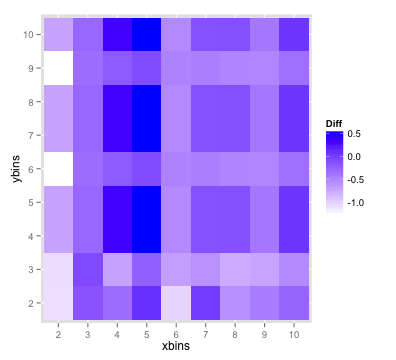
\includegraphics[scale=0.75]{unnamed-chunk-14.png}
\end{center}
\end{figure*}

\section{Distribution of distance
metrics}\label{distribution-of-distance-metrics}

Measuring the quality of a lineup is interesting. But it may also be
important to compare a few lineups. \texttt{"distmet"} function provides
the empirical distribution of the distance metrics based on the mean
distance of the true plot and the mean distance from the null plots. The
lineup data, the null generating mechanism and the choice of the
distance metric has to be provided. Users have the flexibility of using
their distance metrics. The position of the true plot in the lineup has
to be provided as well. If the distance metrics require additional
arguments, those have to be provided as well.

\begin{Shaded}
\begin{Highlighting}[]
\KeywordTok{library}\NormalTok{(ggplot2)}
\NormalTok{lineup.dat <-}\StringTok{ }\KeywordTok{lineup}\NormalTok{(}\KeywordTok{null_permute}\NormalTok{(}\StringTok{'mpg'}\NormalTok{), mtcars, }\DataTypeTok{pos =} \DecValTok{10}\NormalTok{)}
\KeywordTok{qplot}\NormalTok{(mpg, wt, }\DataTypeTok{data =} \NormalTok{lineup.dat, }\DataTypeTok{geom =} \StringTok{'point'}\NormalTok{) +}\StringTok{ }\KeywordTok{facet_wrap}\NormalTok{(~}\StringTok{ }\NormalTok{.sample)}
\end{Highlighting}
\end{Shaded}

Copy and paste the output of lineup.dat to get the position of the true
plot

\begin{Shaded}
\begin{Highlighting}[]
\CommentTok{#decrypt('...') }
\CommentTok{#[1] 'True data in position 10' # Use pos = 10}
\end{Highlighting}
\end{Shaded}

\begin{figure*}[hbtp]
\begin{center}
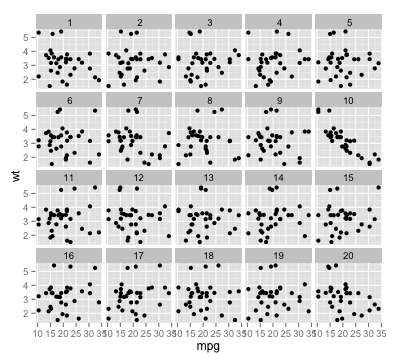
\includegraphics[scale=0.75]{unnamed-chunk-15.png}
\end{center}
\end{figure*}

\begin{Shaded}
\begin{Highlighting}[]
\KeywordTok{library}\NormalTok{(dplyr)}
\NormalTok{dist.vals <-}\StringTok{ }\KeywordTok{distmet}\NormalTok{(lineup.dat, }\DataTypeTok{var =} \KeywordTok{c}\NormalTok{(}\StringTok{'mpg'}\NormalTok{, }\StringTok{'wt'}\NormalTok{),}\StringTok{'reg_dist'}\NormalTok{, }\KeywordTok{null_permute}\NormalTok{(}\StringTok{'mpg'}\NormalTok{), }\\
\DataTypeTok{pos =} \DecValTok{10}\NormalTok{, }\DataTypeTok{repl =} \DecValTok{100}\NormalTok{, }\DataTypeTok{dist.arg =} \OtherTok{NULL}\NormalTok{) }
\end{Highlighting}
\end{Shaded}

\begin{Shaded}
\begin{Highlighting}[]
\KeywordTok{head}\NormalTok{(dist.vals$lineup)}
\end{Highlighting}
\end{Shaded}

\begin{verbatim}
## Source: local data frame [6 x 2]
## 
##   plotno mean.dist
## 1      1    1.2397
## 2      2    0.3427
## 3      3    0.3852
## 4      4    0.6395
## 5      5    0.3387
## 6      6    0.3394
\end{verbatim}

\begin{Shaded}
\begin{Highlighting}[]
\NormalTok{dist.vals$diff}
\end{Highlighting}
\end{Shaded}

\begin{verbatim}
## [1] 6.119
\end{verbatim}

\begin{Shaded}
\begin{Highlighting}[]
\KeywordTok{head}\NormalTok{(dist.vals$closest)}
\end{Highlighting}
\end{Shaded}

\begin{verbatim}
## [1] 20  1  7 17 16
\end{verbatim}

\begin{Shaded}
\begin{Highlighting}[]
\KeywordTok{head}\NormalTok{(dist.vals$null_values)}
\end{Highlighting}
\end{Shaded}

\begin{verbatim}
## [1] 0.6358 0.5557 0.3349 1.2700 0.4673 0.3292
\end{verbatim}

\begin{Shaded}
\begin{Highlighting}[]
\NormalTok{dist.vals$pos}
\end{Highlighting}
\end{Shaded}

\begin{verbatim}
## [1] 10
\end{verbatim}

\begin{Shaded}
\begin{Highlighting}[]
\NormalTok{dist.vals <-}\StringTok{ }\KeywordTok{distmet}\NormalTok{(lineup.dat, }\DataTypeTok{var =} \KeywordTok{c}\NormalTok{(}\StringTok{'mpg'}\NormalTok{, }\StringTok{'wt'}\NormalTok{),}\StringTok{'bin_dist'}\NormalTok{, }\KeywordTok{null_permute}\NormalTok{(}\StringTok{'mpg'}\NormalTok{), } \\
\DataTypeTok{pos =} \DecValTok{10}\NormalTok{, }\DataTypeTok{repl =} \DecValTok{100}\NormalTok{, }\DataTypeTok{dist.arg =} \KeywordTok{list}\NormalTok{(}\DataTypeTok{lineup.dat =} \NormalTok{lineup.dat, }\DataTypeTok{X.bin =} \DecValTok{5}\NormalTok{, }\DataTypeTok{Y.bin =} \DecValTok{5}\NormalTok{)) }
\end{Highlighting}
\end{Shaded}

\section{Plotting the empirical distribution of the distance
metric}\label{plotting-the-empirical-distribution-of-the-distance-metric}

\texttt{"distplot"} functions plots the empirical distribution of the
distance metric, given the output of \texttt{"distmet"} function. The
distribution is shown in grey along the distance for the true plot in
orange and the distances for the null plots in black.

\begin{Shaded}
\begin{Highlighting}[]
\KeywordTok{distplot}\NormalTok{(dist.vals)}
\end{Highlighting}
\end{Shaded}

\begin{figure*}[hbtp]
\begin{center}
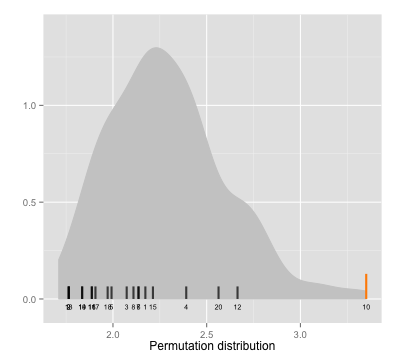
\includegraphics[scale=0.75]{unnamed-chunk-20.png}
\end{center}
\end{figure*}
